\documentclass[../main.tex]{subfiles}
\begin{document}
When we first go for interviews, we may find tree and graph problems intimidating and challenging to solve within 40 mins normal interview window. This might because of our neglinance of the concept of Divide and Conquer or due to the recursion occurrence in tree-related problems. However, at this point, we have already studied the concepts of various trees, divide and conquer, and solved quite a large amount of related questions in previous chapters in this part. We will find out studing this chapter can be real easy compared with the Dynamic programming questions because the consistent principle to solve tree questions.  The principle is to solve problems within \textbf{tree traversal}, either recursively or iteratively,  in either of two ways:  
\begin{enumerate}
    \item \textbf{Top-down Searching}: Tree traversal and with visited nodes information as parameters to be passed to its subtree. The result will be returned from leaf node or empty node, or node that satisfy a certain condition. This is just an extension of the graph search, either BFS or DFS, with recorded path information. This usuallly requires None return from the recursion function, but instead always require a global data structure and a local data structure to track the final answer and the current path information. 
\begin{lstlisting}
def treeTraversalParitial(root, tmp_result):
    if node is empty or node is a leaf node:
        collect the result or return the final result
    construct the previous temp result using the current node
    treeTraversalParitial(root.left, constructured_tmp_result)
    treeTraversalParitial(root.right, constructured_tmp_result)
\end{lstlisting}

\item \textbf{Bottom-up Divide and Conquer:} Due to the special structure of tree, a tree is naturally divided into two halves: left subtree and right subtree. Therefore, we can enforce the Divide and Conquer, to assign two ``agents`` to obtain the result for its subproblems, and back to current node, we ``merge`` the results of the subtree to gain the result for current node. This also requires us to define the return value for edge cases: normally would be empty node and/or leaves.  
\begin{lstlisting}
def treeTraversalDivideConquer(root):
    if node is empty or node is a leaf node:
        return base result
    # divide
    left result = treeTraversalDivideConquer(root.left)
    right result = treeTraversalDivideConquer(root.right)
    
    # conquer
   merge the left and right result with the current node
   return merged result of current node
\end{lstlisting}
\end{enumerate}
The difficulty of these problems are decided by the merge operation, and how many different variables we need to return to decide the next merge operation. However, if we don't like using the recursive function, we can use levelorder traversal implemented with Queue.

Binary tree and Binary Searching tree are the most popular type of questions among interviews. They each take nearly half and half of all the tree questions. We would rarely came into the Segment Tree or Trie, but if you have extra time it will help you learn more if you would study thest two types too.  
\section{Binary Tree (40\%)}
We classify the binary tree related questions as:
\begin{enumerate}
    \item Tree Traversal;
    \item Tree Property: Depth, Height, and Diameter
    \item Tree Advanced Property: LCA 
    \item Tree Path
\end{enumerate}
%%%%%%%%%%%%%%%Tree Traversal%%%%%%%%%%%%%%%%%%%%%%%
\subsection{Tree Traversal}
The problems appearing in this section has mostly been solved in tree traversal section, thus we only list the problems here. 
\begin{enumerate}
    \item 144. Binary Tree Preorder Traversal
    \item 94. Binary Tree Inorder Traversal
    \item 145. Binary Tree Postorder Traversal
    \item 589. N-ary Tree Preorder Traversal
    \item 590. N-ary Tree Postorder Traversal
    \item 429. N-ary Tree Level Order Traversal
    \item 103. Binary Tree Zigzag Level Order Traversal(medium)
    \item 105. Construct Binary Tree from Preorder and Inorder Traversal
\end{enumerate}
\begin{examples}[resume]
\item \textbf{103. Binary Tree Zigzag Level Order Traversal (medium).} Given a binary tree, return the zigzag level order traversal of its nodes' values. (ie, from left to right, then right to left for the next level and alternate between).
\begin{lstlisting}[numbers=none]
For example:
Given binary tree [3,9,20,null,null,15,7],

    3
   / \
  9  20
    /  \
   15   7

return its zigzag level order traversal as:

[
  [3],
  [20,9],
  [15,7]
]
\end{lstlisting}
\textbf{Solution: BFS level order traversal.} We use an variable to track the level of the current queue, and if its even, then we add the result in the original order, otherwise, use the reversed order:
\begin{lstlisting}[language=Python]
def zigzagLevelOrder(self, root):
    """
    :type root: TreeNode
    :rtype: List[List[int]]
    """
    if root is None:
        return []
    q = [root]
    i = 0
    ans = []
    while q:
        tmp = []
        tmpAns = []
        for node in q:
            tmpAns.append(node.val)
            if node.left:
                tmp.append(node.left)
            if node.right:
                tmp.append(node.right)
        q = tmp
        if i % 2 == 0:
            ans += [tmpAns]
        else:
            ans += [tmpAns[::-1]]
        i += 1
    return ans
\end{lstlisting}

\item \textbf{105. Construct Binary Tree from Preorder and Inorder Traversal.} Given preorder and inorder traversal of a tree, construct the binary tree.
Note:You may assume that duplicates do not exist in the tree. 
\begin{lstlisting}[numbers=none]
For example, given preorder = [3,9,20,15,7], inorder = [9,3,15,20,7]
Return the following binary tree:
 
    3
   / \
  9  20
    /  \
   15   7
 \end{lstlisting} 
   
\textbf{Solution: the feature of tree traversal.} The inorder traversal puts the nodes from the left subtree on the left side of root, and the nodes from the right subtree on the right side of the root. While the preorder puts the root at the first place, followed by the left nodes and right nodes. Thus we can find the root node from the preorder, and then use the inorder list to find the root node, and cut the list into two parts: left nodes and right nodes. We use divide and conquer, and do such operation recursively till the preorder and inorder list is empty. 
\begin{lstlisting} [language = Python]
def buildTree(self, preorder, inorder):
        """
        :type preorder: List[int]
        :type inorder: List[int]
        :rtype: TreeNode
        """
        #first to decide the root
        def helper(preorder,inorder):
            if not preorder or not inorder:
                return None
            
            cur_val = preorder[0]
            node = TreeNode(cur_val)
            #divide: now cut the lists into two halfs
            leftinorder,rightinorder = [],[]
            bLeft=True
            for e in inorder:
                if e==cur_val:
                    bLeft=False #switch to the right side
                    continue
                if bLeft:
                    leftinorder.append(e)
                else:
                    rightinorder.append(e)
            leftset, rightset = set(leftinorder),set(rightinorder)
            leftpreorder, rightpreorder = [],[]
            for e in preorder[1:]:
                if e in leftset:
                    leftpreorder.append(e)
                else:
                    rightpreorder.append(e)
                
            #conquer 
            node.left=helper(leftpreorder, leftinorder)
            node.right= helper(rightpreorder,rightinorder)
            return node
        return helper(preorder,inorder)
\end{lstlisting}
However, the previous code has problem as 203 / 203 test cases passed.
Status: Memory Limit Exceeded. So instead of passing new array, I use index.
\begin{lstlisting} [language = Python]
def buildTree(self, preorder, inorder):
        """
        :type preorder: List[int]
        :type inorder: List[int]
        :rtype: TreeNode
        """
        #first to decide the root
        def helper(pre_l, pre_r,in_l, in_r): #[pre_l,pre_r)
            if pre_l>=pre_r  or in_l>=in_r:
                return None
            
            cur_val = preorder[pre_l]
            node = TreeNode(cur_val)
            #divide: now cut the lists into two halfs
            leftinorder = set()
            inorder_index = -1
            for i in range(in_l, in_r):
                if inorder[i]==cur_val:
                    inorder_index = i
                    break
                leftinorder.add(inorder[i])
            #when leftset is empty         
            new_pre_r=pre_l
            for i in range(pre_l+1,pre_r):
                if preorder[i] in leftinorder:
                    new_pre_r = i
                else:
                    break
            new_pre_r+=1         
                
            #conquer 
            node.left=helper(pre_l+1, new_pre_r, in_l, inorder_index)
            node.right= helper(new_pre_r,pre_r, inorder_index+1, in_r)
            return node
        if not preorder or not inorder:
            return None
        return helper(0,len(preorder),0,len(inorder))
\end{lstlisting}


\end{examples}

% 94. Binary Tree Inorder Traversal

% Given a binary tree, return the inorder traversal of its nodes' values.
% \begin{lstlisting}
% Example:

% Input: [1,null,2,3]
%   1
%     \
%      2
%     /
%   3

% Output: [1,3,2]

% Follow up: Recursive solution is trivial, could you do it iteratively?
% \end{lstlisting}
% \begin{lstlisting}[language=Python]
% # recursive
% def inorderTraversal(self, root):
%     """
%     :type root: TreeNode
%     :rtype: List[int]
%     """
%     # left, root, right
%     if root is None:
%         return []
%     left = self.inorderTraversal(root.left)
%     right = self.inorderTraversal(root.right)
%     return left+[root.val]+right
% \end{lstlisting}
% \begin{lstlisting}[language=Python]
% # iterative
% def inorderTraversal(self, root):
%     """
%     :type root: TreeNode
%     :rtype: List[int]
%     """
%     # left, root, right
%     if root is None:
%         return []
%     ans = []
%     stack =[]
%     current = root
%     while current:
%         stack.append(current)
%         current = current.left
%     while stack:
%         tmp = stack.pop()
%         ans.append(tmp.val)
%         current = tmp.right
%         while current:
%             stack.append(current)
%             current = current.left
%     return ans
% \end{lstlisting}

%%%%%%%%%%%%%%%%%%%%%%%Depth%%%%%%%%%%%%%%%%%%%%%%%%%%
\subsection{Depth/Height/Diameter}
In this section, focus on the property related problems of binary tree: including depth, height and diameter. We can be asked to validate balanced binary tree, or the maximum/minimum of these values. The solution is tree traversal along with some operations along can be used to solve this type of problems.
\begin{enumerate}
    \item 111. Minimum Depth of Binary Tree (Easy)
    \item 110. Balanced Binary Tree(Easy)
    \item 543. Diameter of Binary Tree (Easy)
    
    \item 559. Maximum Depth of N-ary Tree (Easy) (Exercise)
    \item 104. Maximum Depth of Binary Tree (Exercise)
\end{enumerate}

\begin{examples}[resume]

\item  \textbf{Minimum Depth of Binary Tree (L111, Easy).} Given a binary tree, find its minimum depth. The minimum depth is the number of nodes along the shortest path from the root node down to the nearest leaf node. \textit{Note: A leaf is a node with no children.}
\begin{lstlisting}
Example:

Given binary tree [3,9,20,null,null,15,7],

    3
   / \
  9  20
    /  \
   15   7

return its minimum depth = 2.
\end{lstlisting}
\textbf{Solution 1: Level-Order Iterative.} For the minumum path, we can traverse the tree level-by-level and once we encounter the first leaf node, this would be the minimum depth and we return from here and has no need to finish traversing the whole tree. The worst time complexity is $O(n)$ and with $O(n)$ space.
\begin{lstlisting}[language=Python]
def minDepth(self, root):
    if root is None:
        return 0
    q = [root]
    d = 0
    while q:
        d += 1
        for node in q:
            if not node.left and not node.right: #a leaf
                return d

        q = [neigbor for n in q for neigbor in [n.left, n.right] if neigbor]           
    return d
\end{lstlisting}
\textbf{Solution 2: DFS + Divide and Conquer.} In this problem, we can still use a DFS based traversal. However, in this solution, without iterating the whole tree we would not get the minimum depth. So, it might take bit longer time. And, this takes $O(h)$ stack space. 
\begin{lstlisting}[language=Python]
def minDepth(self, root):
    if not root:
        return 0
    if not root.left and not root.right: # only leaves will have 1
        return 1
    ans = sys.maxsize
    if root.left:
        ans = min(ans, self.minDepth(root.left))
    if root.right:
        ans = min(ans, self.minDepth(root.right))
    return ans+1
\end{lstlisting}
\item \textbf{110. Balanced Binary Tree(L110, Easy).} Given a binary tree, determine if it is height-balanced. For this problem, a height-balanced binary tree is defined as: \textit{a binary tree in which the \textbf{height} of the two subtrees of every node never differ by more than 1.} (LeetCode used depth however, it should be the height)
\begin{lstlisting}[numbers=none]
Example 1:

Given the following tree [3,9,20,null,null,15,7]:

    3
   / \
  9  20
    /  \
   15   7

Return true.

Example 2:

Given the following tree [1,2,2,3,3,null,null,4,4]:

       1
      / \
     2   2
    / \
   3   3
  / \
 4   4

Return false.
\end{lstlisting}
\textbf{Solution 1: Bottom-up DFS+Divide and conquer with height as return}. First, because the height of a tree is defined as the number of edges on the \textit{longest path} from node to a leaf. And a leaf will have a height of 0. Thus, for the DFS traversal, we need to return 0 for the leaf node, and for an empty node, we use -1 (for leaf node, we have max(-1, -1) + 1 = 0). In this process, we just need to check if the left subtree or the right subtree is already unbalanced which we use -2 to denote, or the difference of the height of the two subtrees is more than 1. 
\begin{lstlisting}[language=Python]
def isBalanced(self, root):
    """
    :type root: TreeNode
    :rtype: bool
    """
    def dfsHeight(root):
        if not root:
            return -1
        lh = dfsHeight(root.left)
        rh = dfsHeight(root.right)
        if lh == -2 or rh == -2 or abs(lh-rh) > 1:
            return -2
        return max(lh, rh)+1
    return dfsHeight(root) != -2
\end{lstlisting}
\item \textbf{543. Diameter of Binary Tree (Easy).} Given a binary tree, you need to compute the length of the diameter of the tree. The diameter of a binary tree is the length of the \textbf{longest} path between any two nodes in a tree. Note: The length of path between two nodes is represented by the number of edges between them. This path may or may not pass through the root.
\begin{lstlisting}[numbers=none]
 Example:
Given a binary tree

          1
         / \
        2   3
       / \     
      4   5    

Return 3, which is the length of the path [4,2,1,3] or [5,2,1,3]. 
\end{lstlisting}
\textbf{Solution: Height of  the tree with global variable to track the diameter.} For node 2, the hegiht should be 1, and the length of path from 4 to 5 is 2, which is sum of the height of 4, 5 and two edges. Thus, we use rootToLeaf to track the height of the subtree. Meanwhile, for each node, we use a global variable to track the maximum path that pass through this node, which we can get from the height of the left subtree and right subtree.
\begin{lstlisting}[language=Python]
def diameterOfBinaryTree(self, root):
    """
    :type root: TreeNode
    :rtype: int
    """
    # this is the longest path from any to any
    
    def rootToAny(root, ans):
        if not root:
            return -1
        left = rootToAny(root.left, ans)
        right = rootToAny(root.right, ans)
        ans[0] = max(ans[0], left+right+2)
        return max(left, right) + 1
    ans = [0]
    rootToAny(root, ans)
    return ans[0]
\end{lstlisting}
\end{examples}
%%%%%%%%%%%%%%%%%%%%Paths%%%%%%%%%%%%%%%%%%%%
\subsection{Paths} 
In this section, we mainly solve path related problems. As we mentioned in Chapter~\ref{chapter_tree}, there are three types of path depending on the starting and ending node type of the path. We might be asked to get minimum/maximum/each path sum/ path length from these three cases: 1) \textbf{root}-to-\textbf{leaf}, 2) \textbf{Root}-to-\textbf{Any} node, 3) \textbf{Any}-node to-\textbf{Any} node. 

Also, maximum or minimum questions is more difficult than the exact path sum, because sometimes when there are negative values in the tree, it makes the situation harder. 

We normally have two ways to solve these problems. One is using DFS traverse and use global variable and current path variable in the parameters of the recursive function to track the path and collect the results.

The second way is DFS and Divide and Conquer, we treat each node as a root tree, we return its result, and for a node, after we get result of left and right subtree, we merge the result. 
%%%%%%%%%%%%%%%%%%%%Root to Leaf Path%%%%%%%%%%%%%%%%%%%%
\subsubsection{Root to Leaf Path}
\begin{enumerate}
    \item 112. Path Sum (Easy)
    \item 113. Path Sum II (easy)
    \item 129. Sum Root to Leaf Numbers (Medium)
    \item 257. Binary Tree Paths (Easy, exer) 
\end{enumerate}
\begin{examples}[resume]
\item \textbf{112. Path Sum (Easy).} Given a binary tree and a sum, determine if the tree has a root-to-leaf path such that adding up all the values along the path equals the given sum. Note: A leaf is a node with no children.
\begin{lstlisting}[numbers=none]
Example:
Given the below binary tree and sum = 22,

      5
     / \
    4   8
   /   / \
  11  13  4
 /  \      \
7    2      1

return true, as there exist a root-to-leaf path 5->4->11->2 which sum is 22.
\end{lstlisting}
\textbf{Solution: Tree Traversal, Leaf Node as Base Case}. Here we are asked the root-to-leaf path sum, we just need to traverse the tree and use the remaining sum after minusing the value of current node to visit its subtree. At the leaf node, if the remaining sum is equal to the node's value, we return True, otherwise False is returned.  Time complexity is $O(n)$.
% is used case The best way to testify the code is to walk through the code with a simple example. For the following example, 1 has no left tree, so the if is None, it should return False for that empty left branch. For any leaf, that is the only place we can possibly return True if the root.val equals to the left sum to need to get. 
% \begin{lstlisting}
%   1
%     \
%      2
% For sum = 1: using the following code will return True
% \end{lstlisting}
\begin{lstlisting}[language=Python]
def hasPathSum(self, root, sum):
    """
    :type root: TreeNode
    :type sum: int
    :rtype: bool
    """
    if root is None: # this is for empty tree
        return False
    if root.left is None and root.right is None: # a leaf as base case
        return True if sum == root.val else False

    left = self.hasPathSum(root.left, sum-root.val)
    if left:
        return True
    right = self.hasPathSum(root.right, sum-root.val)
    if right:
        return True
    return False
\end{lstlisting}
\item \textbf{129. Sum Root to Leaf Numbers (Medium).} Given a binary tree containing digits from 0-9 only, each root-to-leaf path could represent a number. An example is the root-to-leaf path 1->2->3 which represents the number 123. Find the total sum of all root-to-leaf numbers. Note: A leaf is a node with no children.
\begin{lstlisting}[numbers=none]
Example:

Input: [1,2,3,4,5]
     1
    / \
   2   3
  / \
 4   5
Output: 262
Explanation:
The root-to-leaf path 1->2->4 represents the number 124.
The root-to-leaf path 1->2->5 represents the number 125.
The root-to-leaf path 1->3 represents the number 13.
Therefore, sum = 124 + 125 + 13 = 262.
\end{lstlisting}
\textbf{Solution 1: Divide and Conquer.} In divide and conquer solution, we treat each child as a root, for node 4 and 5, they return 4 and 5. For node 2, it should get 24+25, in order to construct this value, the recursive function should return the value of its tree and the path length (number of nodes) of current node to all of its leaf nodes. Therefore for node 2, it has two paths: one with 4, and path length is 1, we get $2*10^(len)$+left, and the same for the right side. The return
\begin{lstlisting}[language=Python]
def sumNumbers(self, root):
    """
    :type root: TreeNode
    :rtype: int
    """
    if not root:
        return 0
    ans, _ = self.sumHelper(root)
    return ans
def sumHelper(self, root):
    if not root:
        return (0, [])
    if root.left is None and root.right is None:
        return (root.val, [1]) # val and depth
    left, ld = self.sumHelper(root.left)
    right, rd = self.sumHelper(root.right)
    # process: sum over the results till this subtree
    ans = left+right
    new_d = []
    for d in ld+rd:
        new_d.append(d+1)
        ans += root.val*10**(d)
    return (ans, new_d)
\end{lstlisting}
\textbf{Solution 2: DFS and Parameter Tracker.} We can also construct the value from top-down, we simply record the path in the tree traversal, and at the end, we simply convert the result to the final answer. 
\begin{lstlisting}[language=Python]
 def sumNumbers(self, root):
        """
        :type root: TreeNode
        :rtype: int
        """
        my_sum = []
        
        self.dfs(root,"",my_sum)
        
        res = 0
        
        for ele in my_sum:
          res += int(ele) # convert a list to an int?
        
        return res
     
    
    def dfs(self,node,routine,my_sum):
      if not node:
        return 
      
      routine = routine + str(node.val)
      if not node.left and not node.right:
        my_sum.append(routine)
        
      self.dfs(node.left,routine,my_sum)
      self.dfs(node.right,routine,my_sum
\end{lstlisting}
\end{examples}
%%%%%%%%%%%%%%%%%%%%%%%%%%Root to Any%%%%%%%%%%%%%%%%%%%%%%%%%%%%%%%%%
\subsubsection{Root to Any Node Path}
%%%%%%%%%%%%%%%%%%%%%%%%%%%%%%%%Any to Any Path%%%%%%%%%%%%%%%%%%%%%%%%%%
\subsubsection{Any to Any Node Path}
In this subsection, we need a concept called Dual Recursive Function. 
\begin{enumerate}
    \item 437. Path Sum III (medium)
    \item 124. Binary Tree Maximum Path Sum (hard)
    \item 543. Diameter of Binary Tree (Easy, put in exercise)
\end{enumerate}
\begin{examples}[resume]
\item \textbf{437. Path Sum III} You are given a binary tree in which each node contains an integer value. Find the number of paths that sum to a given value. The path does not need to start or end at the root or a leaf, but it must go downwards (traveling only from parent nodes to child nodes). The tree has no more than 1,000 nodes and the values are in the range -1,000,000 to 1,000,000.
\begin{lstlisting}[numbers=none]
Example:

root = [10,5,-3,3,2,null,11,3,-2,null,1], sum = 8

      10
     /  \
    5   -3
   / \    \
  3   2   11
 / \   \
3  -2   1

Return 3. The paths that sum to 8 are:

1.  5 -> 3
2.  5 -> 2 -> 1
3. -3 -> 11
\end{lstlisting}
\textbf{Solution 1: Dual Recurrence with Divide and Conquer.} In this problem, it is from any to any node, it is equivalent to finding the root->any with sum for all the nodes in the binary tree. We first write a function for root to any. The complexity is $O(n)$. 
\begin{lstlisting}[language = Python]
def rootToAny(self, root, sum):
    if root is None: 
        return 0
    # collect result at any node
    sum -= root.val
    count = 0
    if sum == 0:
        count += 1
    return count + self.rootToAny(root.left, sum) + self.rootToAny(root.right, sum)
\end{lstlisting}
However, to get the sum of any to any path (downwards),  for each node, we treat it as root node, and call rootToAny, to get satisfactary total paths starts from current node, and we divide the remaining tasks (starting from any other nodes to its left and right subtree).  Thus the time complexity if $O(n^2)$. $n$ subproblems and each takes $O(n)$ time.
\begin{lstlisting}[language = Python]
   '''first recursion: we traverse the tree and use any node as root, and call rootToAny to get its paths'''
def pathSum(self, root, sum):
    if not root:
        return 0

    return self.rootToAny(root, sum) + self.pathSum(root.left, sum) + self.pathSum(root.right, sum)
\end{lstlisting}
\textbf{Solution 2: Optimization with Prefix Sum}. The above solution has large amount of recomputation. This is similar in being in an array: we need to set two pointers, one for subarray start and another for the end. We can use prefix sum to decrease the time complexity to $O(n)$. The sum from n1 to n2 is P[n2]-P[n1] = sum, thus, we need to check P[n1], which equals to P[n2]-sum at each node.  To deal with case: [0,0], sum = 0, we need to add 0:1 into the hashmap. Another difference is: in the tree we are using DFS traversal, for a given node, when we finish visit its left subtree and right subtree, and return to its parent level, we need to reset the hashmap. So, this is DFS with backtracking too.
\begin{lstlisting}[language=Python]
def anyToAnyPreSum(self, root, sum, curr, ans, preSum):
    if root is None: 
        return 
    # process
    curr += root.val
    ans[0] += preSum[curr-sum]
    preSum[curr] += 1
    self.anyToAnyPreSum(root.left, sum, curr, ans, preSum)
    self.anyToAnyPreSum(root.right, sum, curr, ans, preSum)
    preSum[curr] -= 1 #backtrack to current state
    return

def pathSum(self, root, sum):
    if not root:
        return 0
    ans = [0]
    preSum = collections.defaultdict(int)
    preSum[0] = 1
    self.anyToAnyPreSum(root, sum, 0, ans, preSum)
    return ans[0]
\end{lstlisting}
\item \textbf{124. Binary Tree Maximum Path Sum (hard).} Given a non-empty binary tree, find the maximum path sum. For this problem, a path is defined as any sequence of nodes from some starting node to any node in the tree along the parent-child connections. The path must contain at least one node and \textbf{does not need to go through the root}.
\begin{lstlisting}[numbers=none]
Example 1:
Input: [1,2,3]

       1
      / \
     2   3

Output: 6

Example 2:

Input: [-10,9,20,null,null,15,7]

   -10
   / \
  9  20
    /  \
   15   7

Output: 42
\end{lstlisting} 

\textbf{Solution 1: Dual Recurrence}: Before we head over to the optimized solution, first to understand the question. The question can be reparahased as: for each node, find the largest path sum that goes through this node (the path must contain at least one node thus the current node is the one it must include) which is being treated as a root, that is the largest left path sum and the largest right path sum, max(ans[0], max(left, 0)+max(right,0) + root.val). At first, we gain the max path sum from the root to any node, which we implement in the function maxRootToAny. And at the main function, we call maxRootToAny for left and right subtree, then merge the result, then we traverse to the left branch and right branch to do those things too. This is a straightforward dual recurrence. With time complexity $O(n^2)$.
\begin{lstlisting}[language=Python]
def maxRootToAny(self, root):
    if root is None:
        return 0
    left = self.maxRootToAny(root.left)
    right = self.maxRootToAny(root.right)
    # conquer: the current node
    return root.val+max(0, max(left, right)) #if the left and right are both negative, we get rid of it
def maxPathSum(self, root):
    """
    :type root: TreeNode
    :rtype: int
    """
    if root is None:
        return 0
    def helper(root, ans):
        if root is None:
            return
        left = self.maxRootToAny(root.left)
        right = self.maxRootToAny(root.right)
        ans[0] = max(ans[0], max(left, 0)+max(right,0)+root.val)
        helper(root.left, ans)
        helper(root.right, ans)
        return 
    ans = [-sys.maxsize]
    helper(root, ans)
    return ans[0]
\end{lstlisting}
\textbf{Solution 2: Merge the Dual Recurrence}. If we observe these two recurrence function, we can see we use helper(root), we call maxRootToAny with left and right subtree, which is the same as maxRootToAny(root). Then in helper, we use helper(root.left) to call maxRootToAny(root.left.left) and maxRootToAny(root.left.right), which is exactly the same as maxRootToAny(root.left). Thus, the above solution has one power more of complexity. It can be simplied as the following code:
\begin{lstlisting}[language=Python]
def maxRootToAny(self, root, ans):
    if root is None:
        return 0
    left = self.maxRootToAny(root.left, ans)
    right = self.maxRootToAny(root.right, ans)
    ans[0] = max(ans[0], max(left, 0) + max(right,0) + root.val) #track the any->root->any maximum
    # conquer: the current node
    return root.val + max(0, max(left, right)) #track root->any maximum
def maxPathSum(self, root):
    """
    :type root: TreeNode
    :rtype: int
    """
    if root is None:
        return 0
    ans = [-sys.maxsize]
    self.maxRootToAny(root, ans)
    return ans[0]
\end{lstlisting}
The most important two lines of the code is:
\begin{lstlisting}[language=Python]
ans[0] = max(ans[0], max(left, 0) + max(right,0) + root.val) #track the any->root->any maximum
return root.val + max(0, max(left, right)) #track root->any maximum
\end{lstlisting}
\end{examples}
%%%%%%%%%%%%%%%%%%%%Merge%%%%%%%%%%%%%%%%%%%%
\subsection{Reconstruct the Tree}
In this section, we can be asked to rearrange the node or the value of the tree either in-place or out-of-place. Unless be required to do it in-place we can always use the divide and conquer with return value and merge. 
\subsubsection{In-place Reconstruction}
\begin{enumerate}
    \item 114. Flatten Binary Tree to Linked List
\end{enumerate}
\begin{examples}[resume]
\item \textbf{114. Flatten Binary Tree to Linked List (medium).} Given a binary tree, flatten it to a linked list in-place.
\begin{lstlisting}[numbers=none]
For example, given the following tree:

    1
   / \
  2   5
 / \   \
3   4   6

The flattened tree should look like:

1
 \
  2
   \
    3
     \
      4
       \
        5
         \
          6
\end{lstlisting}
\textbf{Solution: Inorder Traversal.} For this, we first notice the flatten rule is to connect node, node.left and node.right, where node.left and node.right is already flatten by the recursive call of the function. For node 2, it will be 2->3->4. First, we need to connect node.right to node.left by setting the last node of the left's right child to be node.right. 
\begin{lstlisting}[language=Python]
def flatten(self, root):
    """
    :type root: TreeNode
    :rtype: void Do not return anything, modify root in-place instead.
    """

    if not root:
        return 
    # preorder
    self.flatten(root.left) # modify root.left
    self.flatten(root.right)

    # traverse the left branch to connect with the right branch
    if root.left is not None:
        node = root.left
        while node.right:
            node = node.right
        node.right = root.right

    else:
        root.left = root.right
    # connet node, left right
    root.right = root.left
    root.left = None
\end{lstlisting}


\end{examples}
\subsubsection{Out-of-place Reconstruction}
\begin{enumerate}
    \item 617. Merge Two Binary Trees
    \item 226. Invert Binary Tree (Easy)
    \item 654. Maximum Binary Tree(Medium)
\end{enumerate}
\begin{examples}[resume]
\item \textbf{617. Merge Two Binary Trees.} Given two binary trees and imagine that when you put one of them to cover the other, some nodes of the two trees are overlapped while the others are not.

You need to merge them into a new binary tree. The merge rule is that if two nodes overlap, then sum node values up as the new value of the merged node. Otherwise, the NOT null node will be used as the node of new tree.
\begin{lstlisting}[numbers=none]
Example 1:
Input: 
	Tree 1                     Tree 2                  
          1                         2     
         / \                       / \              
        3   2                     1   3                  
       /                           \   \                
      5                             4   7                
Output: 
Merged tree:
	     3
	    / \
	   4   5
	  / \   \ 
	 5   4   7

Note: The merging process must start from the root nodes of both trees.
\end{lstlisting}
\textbf{Solution 1: DFS+Divide and Conquer}. In this problem, we just need to traverse these two trees at the same time with the same rule. When both is None which means we just reached a leaf node, we return None for its left and right child. If only one is None, then return the other according to the rule. Otherwise merge their values and assign the left subtree and right subtree to another recursive call and merge all the results to current new node.
\begin{lstlisting}[language=Python]
def mergeTrees(self, t1, t2):
    if t1 is None and t2 is None: # both none
        return None
    if t1 is None and t2:
        return t2
    if t1 and t2 is None:
        return t1
    node = TreeNode(t1.val+t2.val)
    # divide and conquer, left result and the right result
    node.left = self.mergeTrees(t1.left, t2.left)
    node.right = self.mergeTrees(t1.right, t2.right)
    return node
\end{lstlisting}

\item \textbf{226. Invert Binary Tree.} Invert a binary tree.
\begin{lstlisting}[numbers=none]
Example:

Input:

     4
   /   \
  2     7
 / \   / \
1   3 6   9

Output:

     4
   /   \
  7     2
 / \   / \
9   6 3   1
\end{lstlisting}
\textbf{Solution 1: Divide and Conquer}.
\begin{lstlisting}[language=Python]
def invertTree(self, root):
    """
    :type root: TreeNode
    :rtype: TreeNode
    """
    if root is None:
        return None
    
    # divide:  the problem into reversing left subtree and right subtree
    left = self.invertTree(root.left)
    right = self.invertTree(root.right)
    # conquer:  current node
    root.left = right
    root.right = left
    return root
\end{lstlisting}

\item \textbf{654. Maximum Binary Tree.} Given an integer array with no duplicates. A maximum tree building on this array is defined as follow:
 \begin{enumerate}
    \item The root is the maximum number in the array.
    \item The left subtree is the maximum tree constructed from left part subarray divided by the maximum number.
    \item The right subtree is the maximum tree constructed from right part subarray divided by the maximum number.
 \end{enumerate}

Construct the maximum tree by the given array and output the root node of this tree.
\begin{lstlisting}[numbers=none]
Example 1:

Input: [3,2,1,6,0,5]
Output: return the tree root node representing the following tree:

      6
    /   \
   3     5
    \    / 
     2  0   
       \
        1

Note:

    The size of the given array will be in the range [1,1000].

\end{lstlisting}
\textbf{Solution: Divide and Conquer}. The description of the maximum binary tree the root, left subtree, right subtree denotes the root node is the maximum value, and the left child is the max value in the left side of the max value in the array. This fits the divide and conquer. This is so similar as the concept of \textbf{quick sort}. Which divide an array into two halves. The time complexity is $O(nlgn)$. In the worst case, the depth of the recursive tree can grow up to n, which happens in the case of a sorted nums array, giving a complexity of $O(n^2)$.
\begin{lstlisting}[language=Python]
 def constructMaximumBinaryTree(self, nums):
        """
        :type nums: List[int]
        :rtype: TreeNode
        """
        if not nums:
            return None
        (m,i) = max((v,i) for i,v in enumerate(nums)) 
        root = TreeNode(m)
        root.left = self.constructMaximumBinaryTree(nums[:i])
        root.right = self.constructMaximumBinaryTree(nums[i+1:])
        return root
\end{lstlisting}
\textbf{Monotone Queue}. The key idea is:
\begin{enumerate}
    \item We scan numbers from left to right, build the tree one node by one step;
    \item We use a queue to keep some (not all) tree nodes and ensure a decreasing order;
    \item For each number, we keep popping the queue until empty or a bigger number appears; 1) The kicked out smaller number is current node's left child (temporarily, this relationship may change in the future). 2) The bigger number (if exist, it will be still in stack) is current number's parent, this node is the bigger number's right child.  Then we push current number into the stack.
\end{enumerate}
\begin{lstlisting}[language=Python]
def constructMaximumBinaryTree(self, nums):
    """
    :type nums: List[int]
    :rtype: TreeNode
    """
    if not nums:
        return None
    deQ = collections.deque()
    for i, v in enumerate(nums):
        node = TreeNode(v)
        while deQ and deQ[-1].val < v:
            node.left = deQ[-1]
            deQ.pop()
        if deQ:
            deQ[-1].right = node
        deQ.append(node)
    return deQ[0]
\end{lstlisting}
\end{examples}
%%%%%%%%%%%%%%%%%%%%%%%Count%%%%%%%%%%%%%%%%%%%%%%
\subsection{Ad Hoc Problems}
There are some other problems that are flexible and are highly customized requirements. We usually need to be more flexbile with the solutions too. Sometimes, we need to write multiple functions in order to solve one problem. 
\begin{enumerate}
    \item 250. Count Univalue Subtrees
    \item 863. All Nodes Distance K in Binary Tree
\end{enumerate}
\begin{examples}[resume]
\item \textbf{250. Count Univalue Subtrees (medium). } Given a binary tree, count the number of uni-value subtrees. A Uni-value subtree means all nodes of the subtree have the same value.
\begin{lstlisting}[numbers=none]
Example :

Input:  root = [5,1,5,5,5,null,5]

              5
             / \
            1   5
           / \   \
          5   5   5

Output: 4
\end{lstlisting}
\textbf{Solution 1: DFS and Divide and Conquer}. First, all the leaf nodes are univalue subtree with count 1 and also it is the base case with (True, leaf.val, 1) as return. If we are at node 1, we check the left subtree and right subtree if they are univalue, and what is their value, and what is there count. Or for cases that a node only has one subtree. If the val of the subtree and the current node equals, we increase the count by one, and return (True, node.val, l\_count+r\_count+1). All the other cases, we only have (False, None, l\_count+r\_count). 
\begin{lstlisting}[language = Python]
def countUnivalSubtrees(self, root):
    if not root:
        return 0

    def univalSubtree(root):
        if root.left is None and root.right is None:
            return (True, root.val, 1)
        l_uni, l_val, l_count = True, None, 0
        if root.left:
            l_uni, l_val, l_count = univalSubtree(root.left)
        r_uni, r_val, r_count = True, None, 0
        if root.right:
            r_uni, r_val, r_count = univalSubtree(root.right)
        if l_uni and r_uni:
            if l_val is None or r_val is None:# a node with only one subtree
                if l_val == root.val or r_val == root.val:
                    return (True, root.val, l_count+r_count+1)
                else:
                    return (False, None, l_count+r_count)
            if l_val == r_val == root.val: # a node with both subtrees
                return (True, root.val, l_count+r_count+1)
            else:
                return (False, None, l_count+r_count)
        return (False, None, l_count+r_count)
        
    _, _, count = univalSubtree(root)
    return count
\end{lstlisting}
Or else we can use a global variable to record the subtree instead of returning the result from the tree.
\begin{lstlisting}[language=Python]
def countUnivalSubtrees(self, root):
    def helper(root):
        if not root:return True
        if not root.left and not root.right:
            self.res += 1
            return True
        left_res = helper(root.left)
        right_res = helper(root.right)
        if root.left and root.right:    
            if root.val == root.left.val and root.val == root.right.val and left_res and right_res:
                self.res += 1
                return True
            return False
        if root.left and not root.right:
            if root.val == root.left.val and left_res:
                self.res += 1
                return True
            return False
        if root.right and not root.left:
            if root.val == root.right.val and right_res:
                self.res += 1
                return True
            return False
    self.res = 0
    helper(root)
    return self.res
\end{lstlisting}
\item \textbf{863. All Nodes Distance K in Binary Tree (medium).}We are given a binary tree (with root node root), a target node, and an integer value K. (Note that the inputs "root" and "target" are actually TreeNodes.) Return a list of the values of all nodes that have a distance K from the target node.  The answer can be returned in any order.
\begin{lstlisting}[numbers=none]
Example 1:

Input: root = [3,5,1,6,2,0,8,null,null,7,4], target = 5, K = 2
              3
             / \
            5   1
           / \  | \
          6   2 0  8
             / \
            7   4
Output: [7,4,1]

Explanation: 
The nodes that are a distance 2 from the target node (with value 5)
have values 7, 4, and 1.
\end{lstlisting}
\begin{figure}
    \centering
    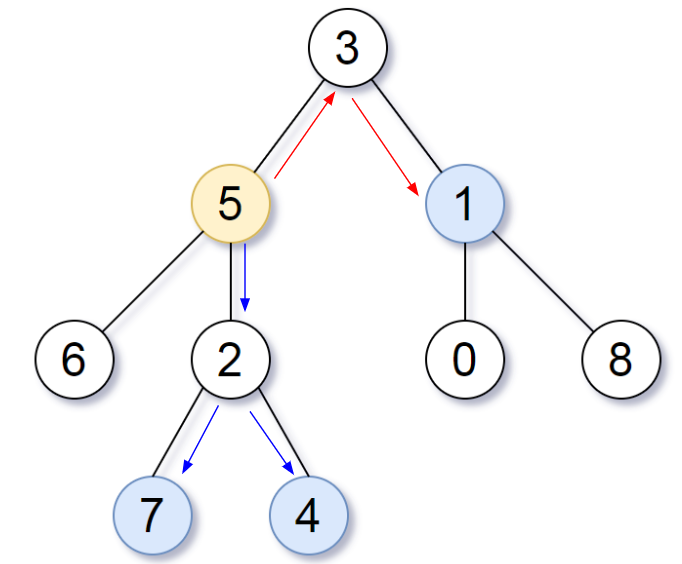
\includegraphics[width=0.7\columnwidth]{fig/example_863.png}
    \caption{Two Cases of K Distance Nodes marked in blue and red arrows. }
    \label{fig:distance_k}
\end{figure}
\textbf{Solution 1: DFS traversal with depth to target as return.} There are different cases with path that has target as denoted in Fig~\ref{fig:distance_k}: 1. target is the starting point, we traverse the target downwards to get nodes that is K distance away from target. 2. target is the ending point, we need to traverse back to its parents, and first check the distance of the parent node with the target to see if it is K, and second we use another function to find K-distance away nodes on the other branch of the parent node. Because we do not have pointer back to its parents directly, we use recursive tree traversal so that we can return to the parent node with its distance to the target. Therefore, we need two helper functions. The first function \textit{getDistanceK} takes a starting node, and a distance K, to return a list of K distance downwards from starting point. The second function \textit{getDepth} is designed to do the above task, when we find the target in the tree traversal, we return 0, for empty node return -1. 
\begin{lstlisting}[language=Python]
def distanceK(self, root, target, K):
    if not root:
        return []
    def getDistanceK(target, K):
        ans = []
        # from target to K distance
        q = [target]
        d = 0
        while q: 
            if d == K:
                ans += [n.val for n in q]
                break
            nq = []
            for n in q:
                if n.left:
                    nq.append(n.left)
                if n.right:
                    nq.append(n.right)
            q = nq
            d += 1
        return ans
        
    # get depth of target
    def getDepth(root, target, K, ans):
        if not root:
            return -1
        if root == target:
            return 0
        # conquer
        left = getDepth(root.left, target, K, ans)
        right = getDepth(root.right, target, K, ans)
        if left == -1 and right == -1:
            return -1
        else:
            dis = 0
            if left != -1:
                dis = left+1
                if root.right:
                    ans += getDistanceK(root.right, K-dis-1)
            else:
                dis = right + 1
                if root.left:
                    ans += getDistanceK(root.left, K-dis-1)
            if dis == K:
                ans.append(root.val)
            return dis
        
    ans = getDistanceK(target, K)
    getDepth(root, target, K, ans)
    return ans
\end{lstlisting}
\textbf{Solution 2: DFS to annotate parent node + BFS to K distance nodes.} In solution 1, we have two cases because we can't traverse to its parents node directly. If we can add the parent node to each node, and the whole tree would become a acyclic direct graph, thus, we can use BFS to find all the nodes that are K distance away. This still has the same complexity.
\begin{lstlisting}[language=Python]
def distanceK(self, root, target, K):
    if not root:
        return []
    def dfs(node, par = None):
        if node is None:
            return
        node.par = par
        dfs(node.left, node)
        dfs(node.right, node)
    dfs(root)
    seen = set([target])
    q = [target]
    d = 0
    while q:
        if d == K:
            return [node.val for node in q]
        nq = []
        for n in q:
            for nei in [n.left, n.right, n.par]:
                if nei and nei not in seen:
                    seen.add(nei)
                    nq.append(nei)
        q = nq
        d += 1
    return []
\end{lstlisting}
\end{examples}



% \begin{enumerate}

% \item Binary Tree Paths
% \begin{inparaenum}
% \item \textbf{Minimum Subtree}
% Given a binary tree, find the subtree with minimum sum. Return the root of the subtree.
% LintCode will print the subtree which root is your return node.

% Solution: we need to get the value of the whole tree, = helper(left)+helper(right)+current val. It’s guaranteed that there is only one subtree with minimum sum and the given binary tree is not an empty tree.

% \item \textbf{The maximum path sum in BT}
% \begin{inparaenum} 
% \item the maximum path sum(root->leaf)

% Example: For the following BT:
% \begin{lstlisting}  
%   1
%  / \
% 2   3
% \end{lstlisting}
% Return 4. (The maximum path is 1->3). However, if we have negative value, this is not going to work.
% \begin{lstlisting} [language = Python]
% public int maxPathSum2(TreeNode root) {
%         if (root == null) {
%             return 0 #th
%         }
%         int left = maxPathSum2(root.left)
%         int right = maxPathSum2(root.right)
        
%         return root.val + Math.max(left, right) #at least root+one of the subtree
%     }
%     \end{lstlisting}
    
% \item the maximum path sum(root->any)

% Binary Tree Maximum Path Sum II, http://www.lintcode.com/zh-cn/problem/binary-tree-maximum-path-sum-ii/

% The path can be from root to any node, but it needs include at least one nod, which is the root.
% Example, For the following BT:
% \begin{lstlisting} 
%   1
%  / \
% 2   3
% \end{lstlisting} 
% Return 4. (Maximum Path is 1->3)

% Solution: this one is slightly different, for each node, we can return the sum of current node +left subtree, or current node+ right subtree, or we just return current node, which means the path ends here.
% For the divide and conquer: 1) Recursive end condition: when the node is null. 2) Divide: divide the tree into the result of the left subtree and right subtree. 3)Conquer: merge the result from the divide.
% \begin{lstlisting} [language = Python]
% public int maxPathSum2(TreeNode root) {
%         if (root == null) {
%             return 0;
%         }
%         //divide
%         int left = maxPathSum2(root.left);
%         int right = maxPathSum2(root.right);
%         //conquer        
%         return root.val + Math.max(0, Math.max(left, right)); #if the max is negative, we get rid of them, use 0 instead.
%     }
% \end{lstlisting}
% \item the maximum path sum(any->any)

% 2.5 Binary Tree Maximum Path Sum


% \end{inparaenum}
% \item Reverse from Traverse result to build tree


% \end{inparaenum}
% \end{enumerate}
% \section{Time complexity of Binary Tree}
% If we spent O(n) to convert $T(n)$ to $2T(n/2)$. We have the following deduction:
% \begin{equation} \label{bt_time}
% \begin{split}
% T(n) & = 2T(n/2) + O(n)\\
%  & = 2 * 2T(n/4) + O(n) + O(n)\\
%  & = O(nlogn)
% \end{split}
% \end{equation}
% which is the same  as merge sort. If the divide cost is only $O(1)$.
% \begin{equation}\label{bt_time2}
% \begin{split}
% T(n) &= 2T(n/2) + O(1)\\
% & = 2 * 2T(n/4) + O(1) + O(1)\\
% &= n + (1 + 2 + 4 +...+ n)\\
% &\approx n + 2n\\
% &\approx O(n)
% \end{split}
% \end{equation}


%%%%%%%%%%%%%%%%%%%%%%%%%%%%%%%%
%%%%BST Related problems and algorithms
%%%%%%%%%%%%%%%%%%%%%%%%%%%%%%%%%%%
\section{Binary Searching Tree (BST)}
\subsection{BST Rules}
\begin{enumerate}
    \item 98. Validate Binary Search Tree (Medium)
    \item 99. Recover Binary Search Tree(hard)
    \item 426. Convert Binary Search Tree to Sorted Doubly Linked List (medium)
\end{enumerate}
\begin{examples}[resume]
\item \textbf{98. Validate Binary Search Tree (medium)} Given a binary tree, determine if it is a valid binary search tree (BST). Assume a BST is defined as follows:
\begin{itemize}
    \item  The left subtree of a node contains only nodes with keys less than the node's key.
    \item The right subtree of a node contains only nodes with keys greater than the node's key.
    \item Both the left and right subtrees must also be binary search trees.
    \end{itemize}
\begin{lstlisting}
Example 1:

Input:
    2
   / \
  1   3
Output: true

Example 2:

    5
   / \
  1   4
     / \
    3   6
Output: false
Explanation: The input is: [5,1,4,null,null,3,6]. The root node's value
             is 5 but its right child's value is 4.
\end{lstlisting}
\textbf{Solution1: Limit the value range for subtrees: top-down}. We start from the root, which should be in range $[-\inf, +\inf]$. And the left subtree should be limited into $[-\inf, root.val]$, and right in $[root.val, +\inf]$. The Code is simple and clean:
\begin{lstlisting}[language=Python]
def isValidBST(self, root, minv=float("-inf"), maxv=float("inf")):
    """
    :type root: TreeNode
    :rtype: bool
    """
    if root is None:
        return True
    
    if (minv < root.val < maxv):
        return self.isValidBST(root.left, minv, root.val) and self.isValidBST(root.right, root.val, maxv)
    return False
\end{lstlisting}
\textbf{Solution 2: Limit the value range for parent node: bottom-up}. We traverse the tree, and we return values from the None node, then we have three cases:
\begin{lstlisting}
1) both subtrees are None # a leaf
     return (True, root.val, root.val)
2) both subtrees are not None: # a subtree with two branches
    check if l2 < root.val < r1:
    merge the range to:
    return (True, l1, r2)
3) one subtree is None: # a subtree with one branches:
   only check one of l2, r1 and merge accordingly
\end{lstlisting}
\textbf{Solution 2: Using inorder}. If we use inorder, then the tree resulting list we obtained should be strictly increasing. 
\begin{lstlisting}[language=Python]
def isValidBST(self, root):
    if root is None:
        return True
    
    def inOrder(root):
        if not root:
            return []
        return inOrder(root.left) + [root.val] + inOrder(root.right)
    ans = inOrder(root)
    pre = float("-inf")
    for v in ans:
        if v <= pre:
            return False
        pre = v
    return True
\end{lstlisting}
\item \textbf{99. Recover Binary Search Tree (hard).} Two elements of a binary search tree (BST) are swapped by mistake. Recover the tree without changing its structure.
\begin{lstlisting}[numbers=none]
Example 1:

Input: [1,3,null,null,2]

   1
  /
 3
  \
   2

Output: [3,1,null,null,2]

   3
  /
 1
  \
   2

Example 2:

Input: [3,1,4,null,null,2]

  3
 / \
1   4
   /
  2

Output: [2,1,4,null,null,3]

  2
 / \
1   4
   /
  3
\end{lstlisting}
Follow up: A solution using O(n) space is pretty straight forward. Could you devise a constant space solution?

\textbf{Solution 1: Recursive InOrder Traversal and Sorting, O(n) space.} The same as validating a BST, the inorder traversal of a valid BST must have a sorted order. Therefore, we obtain the inorder traversed list, and sort them by the node value, and compared the sorted list and the unsorted list to find the  swapped nodes. 
\begin{lstlisting}[language=Python]
def recoverTree(self, root):
    """
    :type root: TreeNode
    :rtype: void Do not return anything, modify root in-place instead.
    """
    def inorder(root):
        if not root:
            return []
        return inorder(root.left) + [root] + inorder(root.right)
    
    
    ans = inorder(root)
    sans = sorted(ans, key = lambda x: x.val)
    # swap 
    for x, y in zip(ans,sans):
        if x != y:
            x.val, y.val = y.val, x.val
            break
\end{lstlisting}
\textbf{Solution 2: Iterative Traversal: O(1) space.} The inorder traversal for each example are:
\begin{lstlisting}[numbers=none]
Example 1: [3, 2, 1], need to switch 3, 1
Example 2: [1, 3, 2, 4], need to switch 3, 2
\end{lstlisting}
If we observe the inorder list: if we check the previous and current pair, if it is dropping as (3,2), (2,1), then we call this dropping pairs. In example 2, there is only one pair (3,2). This is the two possoble cases when we swap a pair of elements  in a sorted list. If we use the inorder iterative traversal, and record the pre, cur dropping pairs, then it is straightforward to do the swapping of the dropping pair or just one pair. 
\begin{lstlisting}[language=Python]
def recoverTree(self, root):
    cur, pre, stack = root, TreeNode(float("-inf")), []
    drops = []
    # inorder iterative: left root, right
    while stack or cur: 
        while cur:
            stack.append(cur)
            cur = cur.left
        cur = stack.pop()
        if cur.val < pre.val:
            drops.append((pre, cur))
        pre, cur = cur, cur.right

    drops[0][0].val, drops[-1][1].val = drops[-1][1].val, drops[0][0].val
\end{lstlisting}
\item \textbf{426. Convert Binary Search Tree to Sorted Doubly Linked List (medium)} Convert a BST to a sorted circular doubly-linked list in-place. Think of the left and right pointers as synonymous to the previous and next pointers in a doubly-linked list. One example is shown in Fig.~\ref{fig:bst_dll}. 
\begin{figure}[h!]
    \centering
    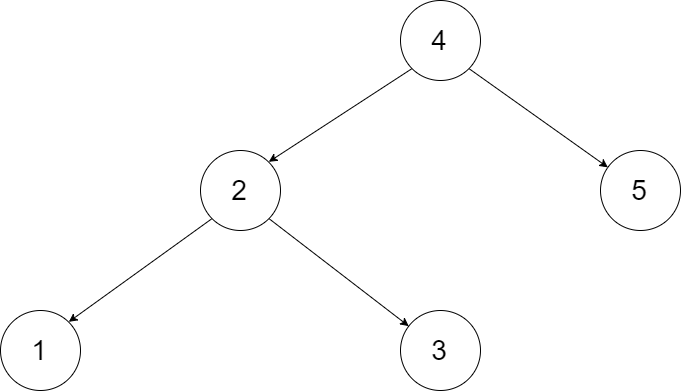
\includegraphics[width=0.45\columnwidth]{fig/bstdlloriginalbst.png}
    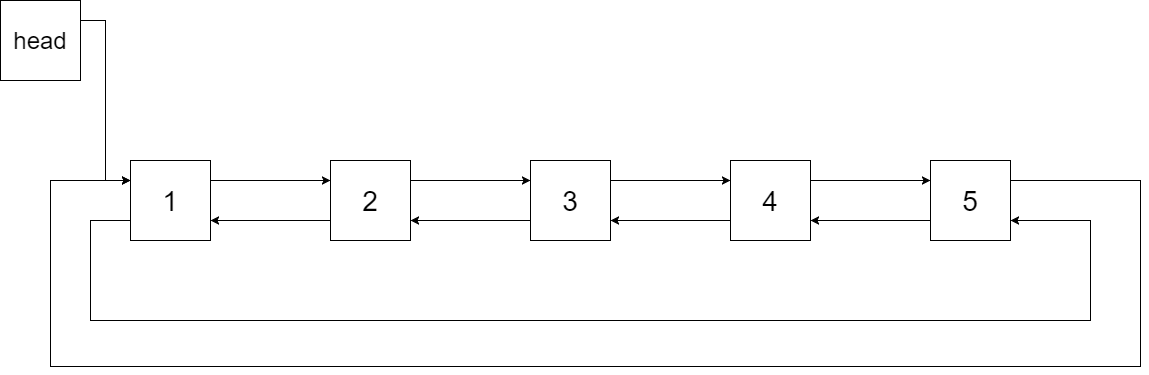
\includegraphics[width=0.45\columnwidth]{fig/bstdllreturndll.png}
    \caption{Example of BST to DLL}
    \label{fig:bst_dll}
\end{figure}

\textbf{Analysis} As we observe the example, for each node in the doubly linked list (dll), its predecessor and successor is the same as the same node in BST. As we have learned the concept of predecessor and successor in Chapter~\ref{chapter_tree}, we know how to find the predecessor and successor individually for each node. However, in this scene, it would be more useful with the inorder traversal, wherein we can use divide and conquer to obtain the left sorted list and the right sorted list for each node. More than this, we need to make the dll, we have two choices to do this: 1) Use our learned inorder traversal to generate a list, and then generate the dll from the list of BST nodes. 2) Combine the inorder traversal together with the linking process.

\textbf{Solution 1: Inorder traversal + Doubly linked List Connect.} This process is straightforward, we need to handle the case where the BST only has one node, or for BST that has at least two nodes. For the second case, we should handle the head and tail node seperately due to its different linking rule:
\begin{lstlisting}[language=Python]
def treeToDoublyList(self, root):
    """
    :type root: Node
    :rtype: Node
    """
    if not root:
        return None
    
    def treeTraversal(root):
        if not root:
            return []          
        left = treeTraversal(root.left)

        right = treeTraversal(root.right)          
        return left + [root] + right
    
    sortList = treeTraversal(root)
    if len(sortList) == 1:
        sortList[0].left = sortList[0]
        sortList[0].right = sortList[0]
        return sortList[0]
    
    for idx, node in enumerate(sortList):
        if idx == 0:
            node.right = sortList[idx+1]
            node.left = sortList[-1]
        elif idx == len(sortList) - 1:
            node.right = sortList[0]
            node.left = sortList[idx-1]
        else:
            node.right = sortList[idx+1]
            node.left = sortList[idx-1]
    return sortList[0] 
\end{lstlisting}

\textbf{Solution 2: Inorder traversal together with linking process.} We use divide and conquer method and assuming the left and right function call gives us the head of the dll on each side. With left\_head and right\_head, we just need to link these two separate dlls with current node in the process of inorder traversal.  The key here is to find the tail left dll, and link them like: left\_tail+current\_node+right\_head, and link left\_head with right\_tail. With dlls, to find the tail from the head, we just need to use head.left. 
\begin{lstlisting}[language=Python]
def treeToDoublyList(self, root):
    """
    :type root: Node
    :rtype: Node
    """
    if not root: return None
    
    left_head = self.treeToDoublyList(root.left)
    right_head = self.treeToDoublyList(root.right)
    return self.concat(left_head, root, right_head)


"""
Concatenate a doubly linked list (prev_head), a node
(curr_node) and a doubly linked list (next_head) into
a new doubly linked list.
"""
def concat(self, left_head, curr_node, right_head):
    # for current node, it has only one node, head and tail is the same
    new_head, new_tail = curr_node, curr_node
    
    if left_head:
        # find left tail
        left_tail = left_head.left 
        # connect tail with current node
        left_tail.right = curr_node
        curr_node.left = left_tail
        # new_head points to left_head
        new_head = left_head  
    
    if right_head:
        right_tail = right_head.left
        # connect head with current node
        curr_node.right = right_head
        right_head.left = curr_node
        new_tail = right_tail # new_tail points to right_tail
    
    new_head.left = new_tail
    new_tail.right = new_head
    return new_head
\end{lstlisting}
\end{examples}

\subsection{Operations} 
In this section, we should problems related to operations we introduced in section~\ref{concept_binary_search_tree}, which include SEARCH, INSERT, GENERATE, DELETE. LeetCode Problems include:
\begin{enumerate}
    \item 108. Convert Sorted Array to Binary Search Tree 
    \item 96. Unique Binary Search Trees
\end{enumerate}

\begin{examples}[resume]
\item \textbf{108. Convert Sorted Array to Binary Search Tree.} Given an array where elements are sorted in ascending order, convert it to a height balanced BST. For this problem, a height-balanced binary tree is defined as a binary tree in which the depth of the two subtrees of every node never differ by more than 1.
\begin{lstlisting}[numbers=none]
Example:

Given the sorted array: [-10,-3,0,5,9],

One possible answer is: [0,-3,9,-10,null,5], which represents the following height balanced BST:
\begin{lstlisting}
      0
     / \
   -3   9
   /   /
 -10  5
\end{lstlisting}

\textbf{Solution: Binary Searching.} use the binary search algorithm, the stop condition is when the l>r.
\begin{lstlisting}[language = Python]
def sortedArrayToBST(self, nums):
        """
        :type nums: List[int]
        :rtype: TreeNode
        """
        def generatebalancedBST(l,r):
            if l>r:
                return None
            m = (l+r)//2
            tree = TreeNode(nums[m])
            tree.left = generatebalancedBST(l,m-1)
            tree.right = generatebalancedBST(m+1,r)
            return tree
        return generatebalancedBST(0,len(nums)-1)
\end{lstlisting}

109. Convert Sorted List to Binary Search Tree, the difference is here we have a linked list, we can convert the linked list into a list nums

\item \textbf{96. Unique Binary Search Trees}

Given n, how many structurally unique BST’s (binary search trees) that store values 1…n?
\begin{lstlisting}[numbers=none]
For example,

 Given n = 3, there are a total of 5 unique BST's.
   1         3     3      2      1
    \       /     /      / \      \
     3     2     1      1   3      2
    /     /       \                 \
   2     1         2                 3
\end{lstlisting}

Solution: When we read the signal, list all of it, we need to use for loop, to pose each element as root, and the left side is left tree, the right side is used for the right tree. Use DPS: We generated all the BST that use ith node as root
\begin{lstlisting}[language = Python]
def numTrees(self, n):
        """
        :type n: int
        :rtype: int
        """ 
        def constructAllBST(start,end):
            if start>end:
                return [None]
            
            #go through the start to end, and use the ith as root
            rslt=[]
            leftsubs,rightsubs=[],[]
            for i in xrange(start,end+1):
                
                leftsubs=constructAllBST(start,i-1)
                rightsubs=constructAllBST(i+1,end)
                for leftnode in leftsubs:
                    for rightnode in rightsubs:
                        node = TreeNode(i)
                        node.left=leftnode
                        node.right=rightnode
                        rslt.append(node)
            return rslt

rslt= constructAllBST(1,n)
        return len(rslt)
        \end{lstlisting}

If we only need length, a slightly better solution showing as follows.
\begin{lstlisting}[language = Python]
def numTrees(self, n):
        """
        :type n: int
        :rtype: int
        """
        def constructAllBST(start,end):
            if start>end:
                return 1
            
            #go through the start to end, and use the ith as root
            count = 0
            leftsubs,rightsubs=[],[]
            for i in xrange(start,end+1):
                
                leftsubs=constructAllBST(start,i-1)
                rightsubs=constructAllBST(i+1,end)
                count+=leftsubs*rightsubs
            return count

rslt= constructAllBST(1,n)
        return rslt
 \end{lstlisting}

However, it still cant pass the test, try the bottom up iterative solution with memorization: $T(start,end)=T(start,i-1)*T(i+1,end) T(j,i)=T(j,i-1)*T(i+1,i)$. How to explain this?
\begin{lstlisting}[language = Python]
def numTrees1(self, n):
    res = [0] * (n+1)
    res[0] = 1
    for i in xrange(1, n+1): #when i=2, j=[0,1] res[2] = res[0]*res[2-1-0] + res[1]*res[2-1-1] 
        for j in xrange(i): #i [1,n], j =[0,i), the case if for one node, 
            res[i] += res[j] * res[i-1-j]
    return res[n]
\end{lstlisting}
Using math:
\begin{lstlisting}[language = Python]
# Catalan Number  (2n)!/((n+1)!*n!)  
def numTrees(self, n):
    return math.factorial(2*n)/(math.factorial(n)*math.factorial(n+1))
\end{lstlisting}

\end{examples}

\subsection{Find certain element of the tree}
successor or predecessor:285. Inorder Successor in BST, 235. Lowest Common Ancestor of a Binary Search Tree
\begin{enumerate} 
    \item 285. Inorder Successor in BST
    \item 235. Lowest Common Ancestor of a Binary Search Tree 
    \item 230. Kth Smallest Element in a BST
    \item 270. Closest Binary Search Tree Value
    \item 272. Closest Binary Search Tree Value II
    \item 426. Convert Binary Search Tree to Sorted Doubly Linked List (find the precessor and successor)
\end{enumerate}
285. Inorder Successor in BST

First, we can follow the definition, use the inorder traverse to get a list of the whole nodes, and we search for the node p and return its next in the lst.
\begin{lstlisting}[language = Python]
#takes 236 ms
def inorderSuccessor(self, root, p):
        """
        :type root: TreeNode
        :type p: TreeNode
        :rtype: TreeNode
        """
        lst = []
        def inorderTravel(node):
            if not node:
                return None
            inorderTravel(node.left)
            lst.append(node)
            inorderTravel(node.right)

        inorderTravel(root)
        
        for i in xrange(len(lst)):
            if lst[i].val==p.val:
                if i+1<len(lst):
                    return lst[i+1]
                else:
                    return None
\end{lstlisting}

However, the definition takes O(N+N), also space complexity is O(N). A slightly better version is when we traverse to find this node, the successor is the last bigger value. So we keep recording the succ
\begin{lstlisting}[language = Python]
#takes 108ms
def inorderSuccessor(self, root, p):
        """
        :type root: TreeNode
        :type p: TreeNode
        :rtype: TreeNode
        """
        #find min(p.right)
        succ = None
        while root:
            if p.val < root.val: #node is bigger than p, go to left
                succ = root #it might be the successor since its bigger
                root = root.left
            else: #node has the same value or smaller value than p, go to right
                root = root.right
        return succ
\end{lstlisting}
235. Lowest Common Ancestor of a Binary Search Tree

Given a binary search tree (BST), find the lowest common ancestor (LCA) of two given nodes in the BST.

According to the definition of LCA on Wikipedia: “The lowest common ancestor is defined between two nodes v and w as the lowest node in T that has both v and w as descendants (where we allow a node to be a descendant of itself).”

For example, the lowest common ancestor (LCA) of nodes 2 and 8 is 6. Another example is LCA of nodes 2 and 4 is 2, since a node can be a descendant of itself according to the LCA definition.

Solution: we traverse the tree to find the first element that is in the range.
\begin{lstlisting}[language = Python]
def lowestCommonAncestor(self, root, p, q):
        """
        :type root: TreeNode
        :type p: TreeNode
        :type q: TreeNode
        :rtype: TreeNode
        """
        s=min(p.val,q.val)
        b=max(p.val,q.val)
        def LCA(node):
            if not node:
                return None
            if node.val>b:
                return LCA(node.left)
            if node.val<s:
                return LCA(node.right)
            return node
            
        return LCA(root)
\end{lstlisting}
230. Kth Smallest Element in a BST

Solution: Here, DFS-inorder-recursive; if we use python, then we need to use list as global variable
\begin{lstlisting}[language = Python]
def kthSmallest(self, root, k):
        """
        :type root: TreeNode
        :type k: int
        :rtype: int
        """
        count = [k] #use list to function as global variable
        num=[-1]
        #inorder traversal
        def inorder(node):
            if node.left:
                inorder(node.left)
            count[0]-=1   #visit         
            if count[0]==0:
                num[0]=node.val
                return
            if node.right:
                inorder(node.right)
        inorder(root)                   
        return num[0]
\end{lstlisting}
Second: DFS iterative
\begin{lstlisting}[language = Python]
def kthSmallest(self, root, k):
        """
        :type root: TreeNode
        :type k: int
        :rtype: int
        """
        count = k
        num=-1
        #DFS iterative
        #1: add all the left nodes
        while root:
            stack.append(root)
            root=root.left
        
        #visit stack, if node.right exist, then add in the stack
        while stack:
            node=stack.pop()
            count-=1
            if count==0:
                return node.val
            #check if the right exist
            right=node.right
            while right:
                stack.append(right)
                right=right.left #keep getting the successor
\end{lstlisting}
270. Closest Binary Search Tree Value

Given a non-empty binary search tree and a target value, find the value in the BST that is closest to the target.

Note:

    Given target value is a floating point.
    
    You are guaranteed to have only one unique value in the BST that is closest to the target.
\begin{lstlisting}[language = Python]
from sys import maxint
class Solution:
    def closestValue(self, root, target):
        """
        :type root: TreeNode
        :type target: float
        :rtype: int
        """
        mind= maxint #current smallest
        rslt= -1
        while root:
            if root.val>target:
                if root.val-target<mind:
                    mind = root.val-target
                    rslt=root.val
                root=root.left
            elif root.val<target:
                if target-root.val<mind:
                    mind = target - root.val
                    rslt=root.val
                root=root.right
            else:
                return root.val
        return rslt
\end{lstlisting}
272. Closest Binary Search Tree Value II
\subsection{Trim the Tree}
maybe with value in the range: 669. Trim a Binary Search Tree

669. Trim a Binary Search Tree

Given a binary search tree and the lowest and highest boundaries as L and R, trim the tree so that all its elements lies in [L, R] (R >= L). You might need to change the root of the tree, so the result should return the new root of the trimmed binary search tree.

Example 2:
\begin{lstlisting}
Input: 
    3
   / \
  0   4
   \
    2
   /
  1

  L = 1
  R = 3

Output: 
      3
     / 
   2   
  /
 1
 \end{lstlisting}

Solution: Based on F1, if the value of current node is smaller than L, suppose at 0, then we delete its left child, node.left = None, then we check its right size, go to node.right, we return node = goto(node.right), if it is within range, then we keep checking left, right, and return current node
\begin{lstlisting}[language = Python]
def trimBST(self, root, L, R):
        """
        :type root: TreeNode
        :type L: int
        :type R: int
        :rtype: TreeNode
        """
        def trimUtil(node):
            if not node:
                return None
            if node.val<L:
                node.left=None #cut the left, the left subtree is definitly smaller than L              
                node =trimUtil(node.right) #node = node.right #check the right
                return node
            elif node.val>R:
                node.right=None
                node=trimUtil(node.left)
                return node
            else:
                node.left=trimUtil(node.left)
                node.right=trimUtil(node.right)
                return node       
        return trimUtil(root)
\end{lstlisting}
A mutant of this is to split the BST into two, one is smaller or equal to the given value, the other is bigger.
\subsection{Split the Tree}
Split the tree

with a certain value ,776. Split BST

776. Split BST

Given a Binary Search Tree (BST) with root node root, and a target value V, split the tree into two subtrees where one subtree has nodes that are all smaller or equal to the target value, while the other subtree has all nodes that are greater than the target value. It's not necessarily the case that the tree contains a node with value V.

Additionally, most of the structure of the original tree should remain. Formally, for any child C with parent P in the original tree, if they are both in the same subtree after the split, then node C should still have the parent P.

You should output the root TreeNode of both subtrees after splitting, in any order.

Example 1:
\begin{lstlisting}
Input: root = [4,2,6,1,3,5,7], V = 2
Output: [[2,1],[4,3,6,null,null,5,7]]
Explanation:
Note that root, output[0], and output[1] are TreeNode objects, not arrays.
\end{lstlisting}

The given tree [4,2,6,1,3,5,7] is represented by the following diagram:
\begin{lstlisting}
          4
        /   \
      2      6
     / \    / \
    1   3  5   7
\end{lstlisting}

Solution: The coding is quite similar as the trimming.
\begin{lstlisting}[language = Python]
class Solution(object):
    def splitBST(self, root, V):
        """
        :type root: TreeNode
        :type V: int
        :rtype: List[TreeNode]
        """
        def splitUtil(node):
            if not node:
                return (None,None)
            if node.val<=V:
                sb1,sb2 = splitUtil(node.right) #the left subtree will satisfy the condition, split the right subtree
                node.right=sb1 #Now set the right subtree with sb1 that
                return (node, sb2)
            else:
                sb1, sb2=splitUtil(node.left) #the right subtree satisfy the condition, split the left subtree
                node.left=sb2
                return (sb1,node)
        return list(splitUtil(root))
\end{lstlisting}

%%%%%%%%%%%%%%%%%%%%%%%%%%%%%%%%%%%%%Exercise%%%%%%%%%%%%%%%%%%%%%%%%%%%%%%%%%%%%%%%%%%%%%%%%%%%%%%%%%%%%
\section{Exercise}
\subsection{Depth}
104. Maximum Depth of Binary Tree (Easy)

Given a binary tree, find its maximum depth. The maximum depth is the number of nodes along the longest path from the root node down to the farthest leaf node.

Note: A leaf is a node with no children.
\begin{lstlisting}
Example:

Given binary tree [3,9,20,null,null,15,7],

    3
   / \
  9  20
    /  \
   15   7

return its depth = 3.
\end{lstlisting}
\textbf{DFS+Divide and conquer}.
\begin{lstlisting}[language=Python]
def maxDepth(self, root):
    if not root:
        return 0
    if not root.left and not root.right:
        return 1
    depth = -sys.maxsize
    if root.left:
        depth = max(depth, self.maxDepth(root.left))
    if root.right:
        depth = max(depth, self.maxDepth(root.right))
    return depth+1 
\end{lstlisting}
559. Maximum Depth of N-ary Tree (Easy)

Given a n-ary tree, find its maximum depth. The maximum depth is the number of nodes along the longest path from the root node down to the farthest leaf node.
\begin{lstlisting}[language=Python]
# Definition for a Node.
class Node(object):
    def __init__(self, val, children):
        self.val = val
        self.children = children

def maxDepth(self, root):
    if not root:
        return 0
    children = root.children
    if not any(children): # a leaf
        return 1
    depth = -sys.maxsize
    for c in children:
        if c:
            depth = max(depth, self.maxDepth(c))
    return depth+1
\end{lstlisting}
%%%%%%%%%%%%%%%%%%%%%%%%%%%Paths%%%%%%%%%%%%%%%%%%%%%%%%%%%%
\subsection{Path}
\textbf{113. Path Sum II (medium).} Given a binary tree and a sum, find all root-to-leaf paths where each path's sum equals the given sum.
\textit{Note: A leaf is a node with no children.}
\begin{lstlisting}[numbers=none]
Example:
Given the below binary tree and sum = 22,

      5
     / \
    4   8
   /   / \
  11  13  4
 /  \    / \
7    2  5   1

Return:

[
   [5,4,11,2],
   [5,8,4,5]
]
\end{lstlisting}
\begin{lstlisting}[language=Python]
def pathSumHelper(self, root, sum, curr, ans):
    if root is None: # this is for one brach tree
        return 
    if root.left is None and root.right is None: # a leaf as base case
        if sum == root.val:
            ans.append(curr+[root.val])
        return

    self.pathSumHelper(root.left, sum-root.val, curr+[root.val], ans)

    self.pathSumHelper(root.right, sum-root.val, curr+[root.val], ans)

def pathSum(self, root, sum):
    """
    :type root: TreeNode
    :type sum: int
    :rtype: List[List[int]]
    """
    ans = []
    self.pathSumhelper(root, sum, [], ans)
    return ans
\end{lstlisting}

257. Binary Tree Paths

Given a binary tree, return all root-to-leaf paths.

Note: A leaf is a node with no children.
\begin{lstlisting}
Example:
Input:

   1
 /   \
2     3
 \
  5
Output: ["1->2->5", "1->3"]
Explanation: All root-to-leaf paths are: 1->2->5, 1->3
\end{lstlisting}
\textbf{Root to Leaf}. Becareful that we only collect result at the leaf, and for the right tree and left tree we need to make sure it is not None:
\begin{lstlisting}[language=Python]
def binaryTreePaths(self, root):
    """
    :type root: TreeNode
    :rtype: List[str]
    """
    def dfs(root, curr, ans):
        if root.left is None and root.right is None: # a leaf
            ans.append(curr+str(root.val))
            return
        if root.left:
            dfs(root.left, curr+str(root.val)+'->', ans)
        if root.right:
            dfs(root.right, curr+str(root.val)+'->', ans)
    if root is None:
        return []
    ans = []
    dfs(root, '', ans)
    return ans
\end{lstlisting}
543. Diameter of Binary Tree

 Given a binary tree, you need to compute the length of the diameter of the tree. The diameter of a binary tree is the length of the longest path between any two nodes in a tree. This path may or may not pass through the root.
\begin{lstlisting}
Example:
Given a binary tree

          1
         / \
        2   3
       / \     
      4   5    

Return 3, which is the length of the path [4,2,1,3] or [5,2,1,3]. 
\end{lstlisting}
\textbf{Root to Any with Global Variable to track the any to any through root}.
\begin{lstlisting}[language=Python]
def diameterOfBinaryTree(self, root):
    """
    :type root: TreeNode
    :rtype: int
    """
    # this is the longest path from any to any
    
    def rootToAny(root, ans):
        if not root:
            return 0
        left = rootToAny(root.left, ans)
        right = rootToAny(root.right, ans)
        ans[0] = max(ans[0], left+right) # track the any to any through root
        return max(left, right) + 1 #get the maximum depth of root to any
    ans = [0]
    rootToAny(root, ans)
    return ans[0]
\end{lstlisting}
% \end{examples}
\end{document}